\chapter{Project plan}
Based on the insight acquired from the previous chapters a plan of approach can be made for the next steps within my research. This will eventually lead to a desired result and a timeline towards this goal. With a summary how this is positioned within the scientific landscape and the key resources.

\section{Desired result}
With the knowledge from the previous chapters a framework can be formed for my research. Hereby taken into account what has already been done and how this can be used.
Although the research consists of two parts. The first part is for the department of Maritime Technology and Transport. The second part of the research will be for the Interactive Intelligence department of computer science. Will the result incorporate the conclusions of both parts, resulting in a single adaption to the bridge system.

This adaption will show the complexity of a situation, which is correlated with te probability of failure. Using a white box approach the hazards. Will there be an overlay for a navigational chart, showing areas with increased risk and an advised sailing route, using different colors. Beside this overlay a list of advised actions will be presented, including the desired operations and communication.

\section{Timeline}
The project is meant to be a full study year, thus 60 ECTS. To have some idea if the project is on schedule, multiple deadlines are set. The planning including these deadlines is presented in table \ref{tab:timeline-project}. This timeline is a rough idea and may be changed during the project depending on new insights or new opportunities.

\begin{table}[h]
	\centering
	\caption{Timeline}
	\label{tab:timeline-project}
	\begin{tabular}{l||l|l}
		Bescrhijving & Start & Deadline \\ \hline \hline
		Project plan met initiele planning &  & 6 okt \\ \hline
		Samenvatting gerelateerde projecten en onderzoeken & 4 okt & 20 okt \\ \hline
		Plan van aanpak met opzet voor rapport & 9 okt & 3 nov \\ \hline
		Inlezen in papers en projecten en vertalen naar current knowledge & 20 okt & 19 nov \\ \hline
		Definieer well-clear op basis van regulations en company policy & 1 nov & 19 nov \\ \hline
		Plan van aanpak definitief maken & 20 nov & 26 nov \\ \hline
		Programma van eisen voor tool opstellen en test voor CS & 26 nov & 17 dec \\ \hline
		Onderzoek naar cost functie en modellen benodigd vanuit MT perspectief & 17 dec & 10 feb \\ \hline
		Opzet voor onderzoek met crew & 5 feb & 10 feb \\ \hline
		Ontwikkelen van GUI en tool op basis van programma van eisen & 12 feb & 5 mar \\ \hline
		Testen met crew & 5 mar & 2 apr \\ \hline
		Tool verbeteren op plekken waar meer detail nodig is & 19 mar & 6 apr \\ \hline
		Opnieuw testen en vergelijken met eerdere tests & 2 apr & 13 apr \\ \hline
		Vergelijking maken tussen theorie en praktijk & 16 apr & 30 apr \\ \hline
		Rapport CS en MT finaliseren & 30 apr & 4 jun \\ \hline
		Artikel schrijven & 4 jun & 29 jun \\ \hline
		Presentatie & 24 jun & 6 jul
	\end{tabular}
\end{table}

\section{Research questions}
Using the information gathered in the previous chapters, a step can be made towards a clear definition of the thesis statement. The initial starting point is written down as an open question. This is done for both the maritime technology part and the computer science part:
\begin{quote}
	\emph{Maritime Technology}\\
	How will insight into the probability of failure and complexity of a situation, help to determine the well-clear condition for different ship types and situations, which improves the advise on potential hazards and safe area's by bridge systems?
\end{quote}

\begin{quote}
	\emph{Computer Science}\\
	Why does the shipping crew acquire situational awareness faster, when receiving information on potential hazards and safe sailing area's, instead of only using traditional bridge sensors?
\end{quote}

Beside these main questions, other questions have to be answered to give a well founded answer on the main questions. Those questions can be answered using literature, interviews, but in some cases are models developed, which might be used in the final model. These questions will be the basis for the reports. 

\begin{itemize}
	\item What is needed to create situation awareness?
	\item What information is available at the bridge?
	\item Which information is available trough authorities?
	\item Which information is shared and communicated between different vessels?
	\item How can this information be stored and used in the model?
	\item What are in general the possible choices of the crew?
	\item What is the probability that certain choices are made?\\
	
	\item What is done well while supporting navigation?
	\item Where are mistakes made during navigation?
	\item How are regulations influencing the development of safer bridge systems?\\

	\item What determines the manoeuvrability of a ship and can this be classified using estimations?
	\item What is the uncertainty of the physical models?
	\item Which information should be visualized?
\end{itemize}

%Thesis statements
%MT: Adapting the well-clear condition to different ship types and situations will enable bridge systems to give a clearer advise on potential hazards and safe area's. 

%CS: Shipping crew will acquire situational awareness faster, when receiving information on potential hazards and safe sailing area's, instead of using traditional bridge sensors

\newpage
\section{Scope}
Due to the time limits and the way this project is set-up. Not everything will be taken into account. The focus will be to improve the availability of information on hazards and safe area's. Developing a model providing the information, and developing a tool to present the information. 

\subsection{Model}
The overlay for the chart system is based on the model for complexity. To determine the complexity certain steps are taken. In those steps some parts are assumed. General assumptions are a 3 \ac{DOF} system, no shallow water, no ship-ship or ship-bank interaction and no extreme movements. This is done to simplify the calculations. Beside these assumptions, during the different phases the model goes trough, assumptions will be made too. 
\begin{enumerate}
	\item \emph{Determine future locations after a number of time intervals:}\\
	For every dynamic object tracks are calculated. The current speed trough water is used, later this can be extended with the acceleration. For every rudder angle the rate of turn is determined and thus the change of heading. On every track the speed and change of heading is kept constant. A normal distribution for the chosen rudder angle is used, to calculate if a certain track is chosen, as the least amount of change is desired. Manoeuvrability estimations are needed for the different dynamic objects.
	\item \emph{Find collision points, based on tracks}\\
	Based on the tracks, a probability for collision at a certain point can be determined. Depending on the current situation, the well-clear distance can be set.
	\item \emph{Determine how hard it is to avoid collision:}\\
	This is done by changing speed. Data on inertia of object is needed. Most efficient when least amount of changes are made. The first iteration will focus on avoidance, not taking into account to get back on track, nor zigzagging or other extreme movements.
	\item \emph{Update probabilities:}\\
	Using information from collision avoidance system and regulations. 
	\item \emph{Determine safe area:}\\
	Subtracting forbidden area's, risk area's. If circles are used, the advised route is perpendicular with that circle. 	
\end{enumerate}

\subsection{Tool}
The tool which uses the information from the model will have the overlay function. This tool will be developed for the crew, whom are directly responsible for navigation. Usually this is the captain. Therefore he will be the main focus during the first iterative step. Before setting the exact scope of this part, the impact and tasks of the captain have to be mapped.

\newpage
\subsection{Chosen vessels and situations}
The tool will be tested for ships of different sizes, this is done to get insight in the effect of manoeuvrability. For now three ships are chosen where much data is available for, there characteristics are shown below and photos in figure \ref{fig:vessels}:

\begin{tabular}[L]{l l}
	Name			& BIBBY WAVEMASTER 1 \\
	Type			& Service Operations Vessel \\
	Length o.a.		& 90.00 m \\
	Beam mld.		& 20.00 m \\
	Design draught	& 4.80 m \\
	Deadweight		& 2400 t \\
	Speed			& 13 kn \\
	& \\
	Name			& DAMEN ASD 2810 \\
	Type			& Tug \\
	Length o.a.		& 28.67	m \\
	Beam mld.		& 10.34	m \\
	Design draught	& 4.72 m \\
	Deadweight		& 531 t \\
	Speed			& 13.8 kn \\
	& \\
	Name			& KRISO Very Large Crude Carrier 2 \\
	Type			& Academic standard model oil tanker\\
	Length o.a.		& 320.0 m \\
	Beam mld.		& 58.0 m \\
	Design draught	& 20.8 m \\
	Deadweight		& 320438 ton \\
	Speed			& 7.97 kn \\
\end{tabular}

Other vessels which do occur in the different situations are classified according to navigational regulations, their size and displacement. The list with these types of vessels will be defined later in the project. Combined with more relevant characteristics for the previously mentioned vessels.

For the analysis different situations will be tested. Together with Marin can be discussed which are relevant. The collision between the FLINTERSTAR and AL ORAIQ is a good example, other situations might also be based on previous accidents.

\begin{figure}[H]
	\centering
	
	\begin{subfigure}[b]{0.3\textwidth}
		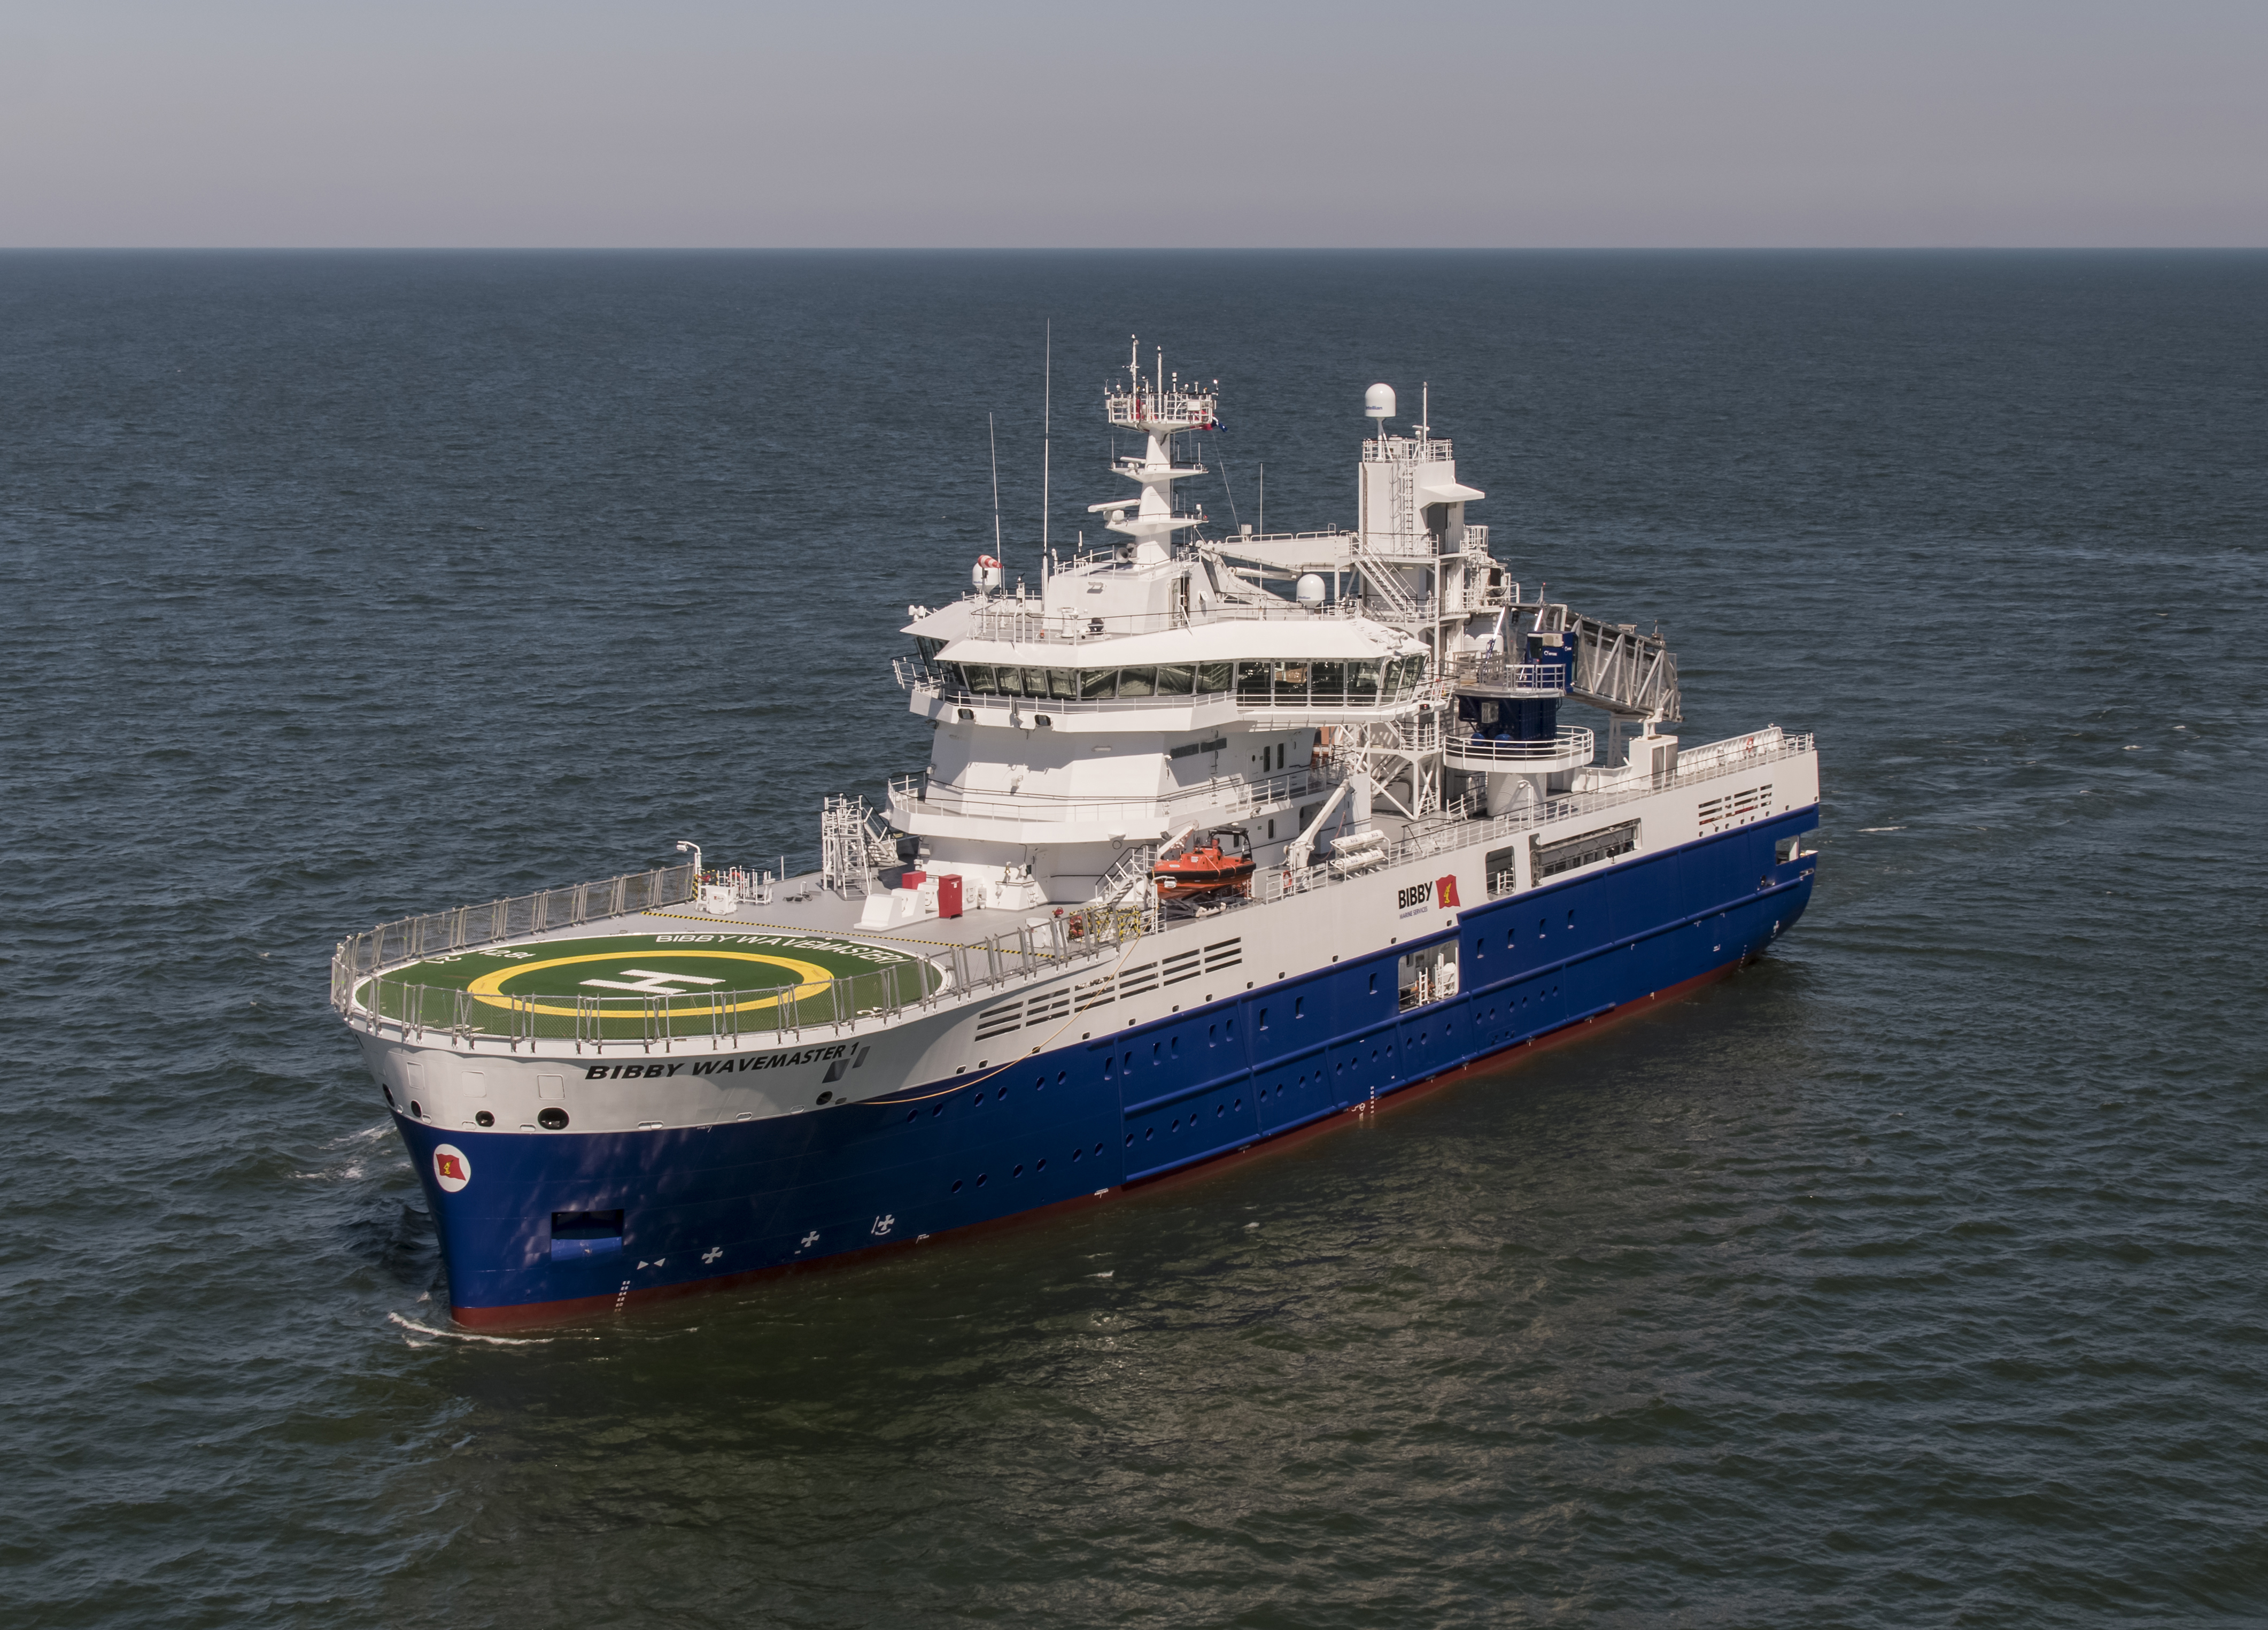
\includegraphics[height=3.5cm, keepaspectratio]{BIBBY-WAVEMASTER-1.jpg}
		\caption{BIBBY WAVEMASTER 1}
	\end{subfigure}
	\hfill
	\begin{subfigure}[b]{0.3\textwidth}
		\includegraphics[height=3.5cm, keepaspectratio]{DAMEN-ASD-TUG-2810.JPG}
		\caption{DAMEN ASD Tug 2810}
	\end{subfigure}
	\hfill
	\begin{subfigure}[b]{0.3\textwidth}
		\includegraphics[height=3.5cm, keepaspectratio]{SIRIUS-STAR.jpg}
		\caption{SIRIUS STAR}
	\end{subfigure}	
	
	\caption{Vessel to be used}
	\label{fig:vessels}
	
\end{figure}